\documentclass[a4paper,14pt]{extarticle}
\usepackage[T2A]{fontenc}
\usepackage[english, russian]{babel}
\usepackage[utf8]{inputenc}
\usepackage{subfiles}
\usepackage{ucs}
\usepackage{textcomp}
\usepackage{array}
\usepackage{indentfirst}
\usepackage{amsmath}
\usepackage{amssymb}
\usepackage{enumerate}
\usepackage[margin=1.5cm,left=2cm,right=2cm,top=3cm,bottom=3cm]{geometry}
\usepackage{authblk}
\usepackage{tikz}
\usepackage{icomma}
\usepackage{gensymb}
\usepackage{subfigure}
\usepackage{algorithm}
\usepackage{algpseudocode}

\title{Отчёт об исследовательской работе по теме \\
<<AI for Automatic Algorithm Synthesis>>}
\author{Студент: Игорь Ельчинов (БПМИ 251) \and Научный руководитель: Рамон Антонио Родригес Залепинос}


\date{Москва, 2025}

\begin{document}


\maketitle

\newpage

\tableofcontents

\newpage
\section{Введение}
    Автоматическое машинное обучение~--- это раздел машинного обучения, который ставит своей целью создание алгоритмов для решения конкретной задачи или их частей с как можно меньшим участием человека.

    В 2010х годах глубокое обучение позволило достичь больших успехов в таких областях, как классификация изображений, поиск объектов на изображении и моделирование языка.
    Несмотря на все достижения, существенным недостатком новых моделей является ручной процесс их разработки методом проб и ошибок, что означает, что даже экспертам требуется много времени и ресурсов на разработку качественных моделей.
    Чтобы сократить издержки была предложена идея автоматизировать весь процесс разработки моделей (автоматическое машинное обучение, automated machine learning, AutoML).
    AutoML позволяет снизить нагрузку на дата-саентистов и применять МО на практике, не имея больших знаний статистики или машинного обучения. 

    После того как в статье \cite{bibl:first-automl} было показано, что автоматически можно генерировать алгоритмы, не уступающие аналогам, сделанным людьми, начался взрывной рост исследований в области поиска нейросетевых архитектур (Neural Architecture Search, NAS).
    Суть NAS заключается в поиске эффективных архитектур нейронных сетей за счёт комбинирования базовых операций, задающих пространство поиска.

    Далее мы подробно рассмотрим несколько работ из области автоматического машинного обучения.
    Сначала мы рассмотрим обзорную статью 2021 года~\cite{bibl:sota}, которая перечисляет <<классические>> подходы в AutoML.
    Далее будет рассмотрен один из таких подходов, описанный в статье~\cite{bibl:evolved-transformer}.
    Затем будут рассмотрены две статьи (\cite{bibl:az}, \cite{bibl:moaz}), подход которых заключается в генерации алгоритмов машинного обучения целиком <<с чистого листа>> с использованием программ на псевдокоде в качестве пространства поиска.
    После будут рассмотрены две статьи (\cite{bibl:shinkaevolve}, \cite{bibl:alphaevolve}), предлагающие использовать большие языковые модели для внесения правок в генерируемую программу и управления процессом эволюции.
    Мы завершим рассмотрением статьи \cite{bibl:adas}, где предлагается использовать автоматическое машинное обучение для генерации сложных объектов, а именно целых агентов.

    Затем будут рассмотрены основные датасеты и бенчмарки, используемые в AutoML, один из которых будет рассмотрен подробнее.
    В конце, на основе всех рассмотренных статей, будет поставлена задача исследования, а также сформулирован план дальнейшей работы.

\newpage
\section{Обзор литературы}
\subsection{AutoML: A Survey of the State-of-the-Art}
    Процесс разработки модели можно разделить на следующие этапы: подготовка данных, инженерия признаков (feature engineering), генерация модели и оценка качества её работы.
    Генерация модели может быть далее разделена на пространство поиска (т.е. принципы, на основе которых будет строиться модель) и методы оптимизации (оптимизация гиперпараметров и оптимизация архитектуры модели).
    Поиск нейросетевых архитектур (Neural Architecture Search, NAS) состоит из трёх главных составляющих: пространства поиска, методов оптимизации и методов оценки полученной архитектуры.
    В данной статье авторы рассматривают передовые методы в AutoML на всех этапах разработки модели.

    \textbf{Подготовка данных.}
    Первым этапом является подготовка данных, которая включает в себя сбор, очистку и аугментацию.
    
    Для некоторых задач, например, классификации изображений, есть хорошие открытые датасеты, однако для других задач данных может быть меньше, или работа с ними может быть затруднена из-за их персонального характера (например, задача классификации медицинских снимков). 
    Поэтому вместо поиска данных в интернете некоторые исследователи предлагают их генерировать.

    Для некоторых задач, особенно связанных с обучением с подкреплением (например, автономный транспорт), возможно использовать симуляторы.
    В открытом доступе есть такие инструменты, как OpenAI Gym (source?), которые позволяют исследователям сосредоточиться на разработке алгоритма, а не на поиске данных.
    Для других задач было предложено использовать генеративные состязательные сети для генерации синтетических данных.

    Полученные данные содержат шумы, которые должны быть очищены. Было предложено несколько алгоритмов, например, BoostClean и AlphaClean, для автоматизации этого процесса.
    Однако их недостатком является применимость только в рамках конкретного датасета.
    Авторы статей \cite{bibl:clean1} и \cite{bibl:clean2} предлагают решения для очистки данных, которые могут использовать знания из предыдущих датасетов для обработки новых.

    Аугментация данных служит регуляризатором, предотвращающим переобучение моделей.
    Для задач компьютерного зрения традиционно использовались простые трансформации (например, отзеркаливание), но некоторые исследователи предлагают использовать нейронные сети для аугментации изображений.
    Для текстовых данных используется замена слов на синонимичные или последовательный перевод текста между несколькими языками.
    Недостатками этих подходов является зависимость от человеческого знания.
    Чтобы исправить эту проблему, был предложен алгоритм AutoAugment, однако он требует большого числа вычислительных ресурсов.

    \textbf{Инженерия признаков (Feature Engineering).}
    Данный этап обычно делится на отбор признаков (feature selection), построение признаков (feature construction) и извлечение признаков (feature extraction).

    Отбор признаков используется для построения меньшего набора признаков за счёт отбора действительно существенных признаков.
    Основными методами поиска здесь являются полный перебор, случайный перебор и перебор на основе евристик.
    Наиболее частыми методами случайного поиска являются симуляция отжига и эволюционные алгоритмы.

    Построение признаков~--- это процесс, который создаёт новые признаки на основе комбинаций и преобразований старых.
    Так как перебрать все варианты вручную невозможно, были предложены алгоритмы, которые позволяют автоматизировать этот процесс.
    Самыми частыми методами являются решающие деревья, генетические алгоритмы и подходы, основанные на примечаниях.
    Последние обладают преимуществом, так как не требуют заранее определённого пространства преобразований.

    Извлечение признаков позволяет уменьшить количество признаков.
    В отличие от отбора признаков, здесь исходные признаки также изменяются.
    Наиболее эффективными подходами в этой области являются PCA и LDA.
    Недавно также приобрёл популярность подход, который обучает нейронную сеть и использует состояния её внутренних слоёв как новые признаки.

    \textbf{Генерация модели: пространство поиска.}

    \begin{figure}[t]
        \centering
        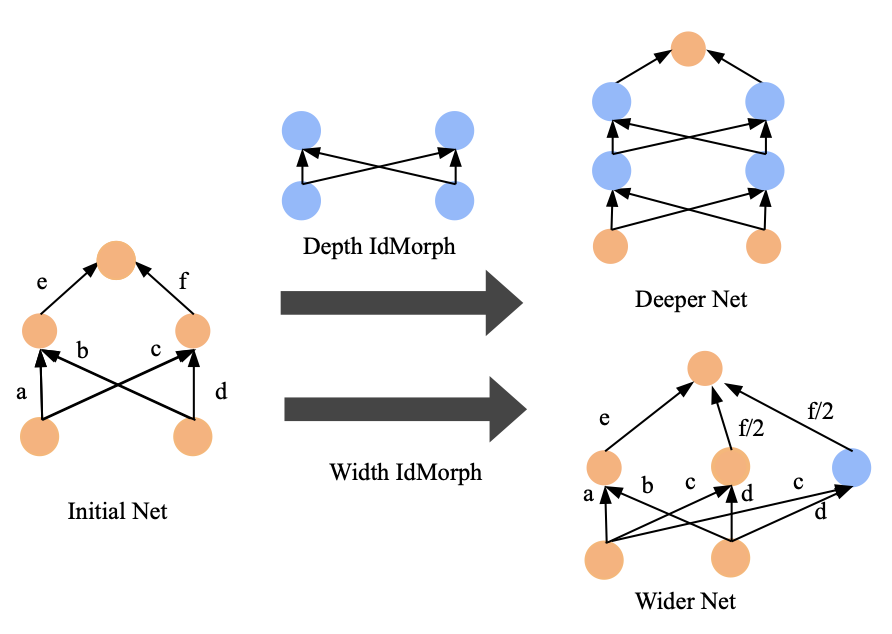
\includegraphics[width=0.4\linewidth]{morphism-operation-example.png}
        \caption{Пример операций identity morphism transformations для morphism-based search space.~\cite{bibl:sota}}
        \label{fig:sota-morphism}
    \end{figure}
    
    Пространство поиска задаёт принципы, на основе которых строится архитектура модели.
    Зачастую методы NAS строят нейросеть как комбинацию простых блоков, созданных людьми (например, разные виды свёрток).
    Ниже будут рассмотрены основные виды пространства поиска.

    \emph{Полное пространство поиска.}
    Хотя данный подход накладывает наименьшие ограничения на архитектуру модели и прост в реализации, его существенным недостатком является большие вычислительные затраты.

    \emph{Ячеистое пространство поиска (Sell-based search space).}
    Данный подход основывается на наблюдении, что большинство успешных нейронных сетей используют некоторые блоки, которые затем последовательно объединяются в итоговую сеть.
    Так как теперь задача сводится к поиску оптимальной архитектуры одного блока, а не всей сети, этот подход требует значительно меньше вычислительных ресурсов.
    Однако и у этого метода есть свои недостатки, например, для обучения и оценки модели зачастую используется сеть с разным числом блоков, что может искажать результаты.
    Такие методы, как progressive-DARTS решают эту проблему за счёт большего числа итераций обучения с постепенным увеличением числа блоков.
    Эксперименты показывают, что этот метод позволяет генерировать нейронные сети с 2.50\% ошибочных предсказаний на датасете CIFAR-10.

    \emph{Иерархическое пространство поиска.}
    Ещё один недостаток предыдущего подхода заключается в том, что он концентрируется на архиректуре отдельного блока, игнорируя архитектуру всей сети.
    Такие параметры, как количество блоков, всё ещё должны настраиваться вручную.
    Чтобы решить эту проблему, был предложен метод HierNAS, где блок более высокого уровня собирается как комбинация блоков предыдущего уровня.

    \emph{Морфическое пространство (Morphism-based Search Space).}
    Данный подход основывается на идее передачи заний от одной модели к другой.
    Такие методы как дистилляция и transfer learning не позволяют перенести архитектуру модели, поэтому была предложена техника Net2Net.
    Он использует операции identity morphism transformations, чтобы строить на основе исходной модели идентичную, но с большим числом слоёв или с увеличенными слоями.
    Улучшенный метод network morphism \cite{bibl:morphism} был предложен, чтобы исправить недостатки предыдущего подхода.
    Он позволяет дочерней нейронной сети унаследовать всё знание от родительской и продолжать развиваться дальше за значительно меньшее время.

    \textbf{Генерация модели: методы оптимизации.}
    После того как было определено пространство поиска, необходимо выбрать метод, с помощью которого будет найдена оптимальная архитектура.
    Здесь будут рассмотрены основные подходы.

    \begin{figure}[t]
        \centering
        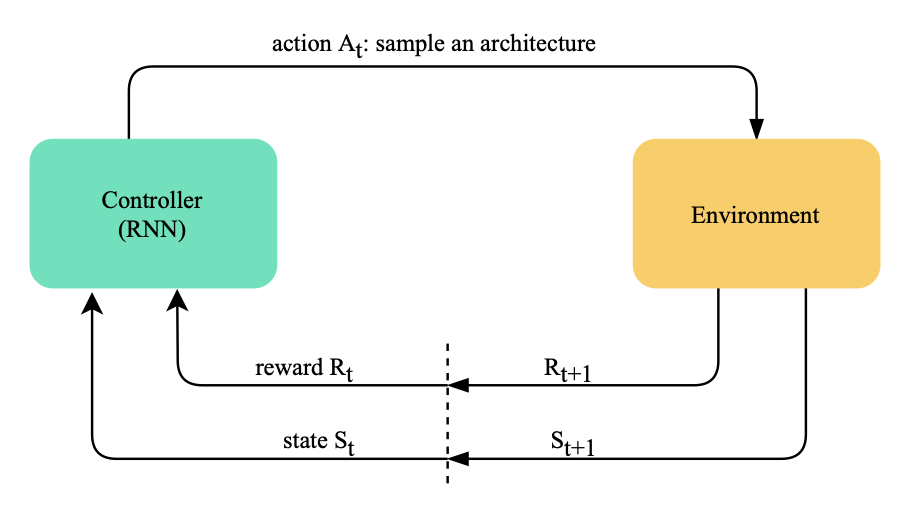
\includegraphics[width=0.5\linewidth]{rl-based-nas.png}
        \caption{Схема работы обучения с подкреплением для генерации архитектуры нейронной сети.~\cite{bibl:sota}}
        \label{fig:rl-based-nas}
    \end{figure}

    \emph{Эволюционные алгоритмы.}
    Данный тип алгоритмов вдохновлён природной эволюцией.
    Для начала выбирается способ представления архитектуры нейронной сети, удобный для изменения и рекомбинации.
    Основными подходами являются DAG, GDP и Cellular encoding.
    Большинство эволюционных алгоритмов состоит из 4 шагов:
    \begin{itemize}
        \item Отбор. На этом этапе из всех ранее найденных архитектур отсеиваются слабые, чтобы остальные можно было использовать для стадии скрещивания. Основными методами являются отбор по приспособленности (fitness selection), отбор по рангу (rank selection) (для отбора кандидатов используется абсолютная и относительная точность соответственно) и турнирный отбор (tournament selection).

        \item Скрещивание. На этом этапе каждая пара выбранных кандидатов формирует потомство, наследующее половину генетической информации от каждого из родителей. Конкретный метод рекомбинации зависит от выбранного  способа представления архитектуры нейронной сети.

        \item Мутация. После рекомбинации в полученную архитектуру вносятся случайные изменения, которые могут приводить как к потере работоспособности архитектуры, так и к поиску новых подходов.

        \item Обновление популяции. Так как в процессе алгоритма генерируется большое количество новых архитектур, популяцию необходимо обновлять, удаляя старые архитектуры по некоторому правилу.
    \end{itemize}

    \emph{Обучение с подкреплением.} 
    Впервые использование обучения с подкреплением для генерации архитектур было предложено в статье \cite{bibl:rlautoml}.
    Здесь контроллер (рекуррентная нейронная сеть) в каждый момент времени выполняет действие, порождающее новую архитектуру, и получает в ответ информацию о текущем состоянии среды (процесс обучения выбранной архитектуры) и функцию награды (точность полученной модели).
    На основе этой работы было предложено множество схожих подходов.
    Хотя обучение с подкреплением позволяет добиться выдающихся результатов в плане точности получаемой модели, оно слишком ресурсозатратно.
    Чтобы справиться с этой проблемой были предложены новые алгоритмы, например, BlockQNN и ENAS, которые используют асинхронное обучение и разделение параметров между всеми полученными архитектурами, чтобы ускорить генерацию модели.


    \emph{Градиентный спуск.}
    В отличие от предыдущих подходов, использующих дискретное пространство поиска, алгоритм DARTS использует градиентный спуск для поиска архитектуры в непрерывном дифференцируемом пространстве поиска.
    Здесь связь между узлами сети осуществляется с помощью взвешенной суммы всех операций-кандидатов.
    В процессе обучения веса операций меняются.
    Финальная архитектура задаётся операциями с наибольшим весом на момент окончания поиска.
    Недостатком такого подхода является большая вычислительная сложность, что особенно важно, линейная зависимость сложности от числа операций-кандидатов.
    Дальнейшие алгоритмы (GDAS, ProxylessNAS) предложили способы сократить количество вычислений.
    Ещё одной проблемой является вероятность того, что операции-кандидаты будут соперничать друг с другом.
    Эта проблема была решена в алгоритме DARTS+ с помощью остановки обучения, если нежелательные операции (например, skip-connection) начинают доминировать в сети.

    \begin{figure}[t]
        \centering
        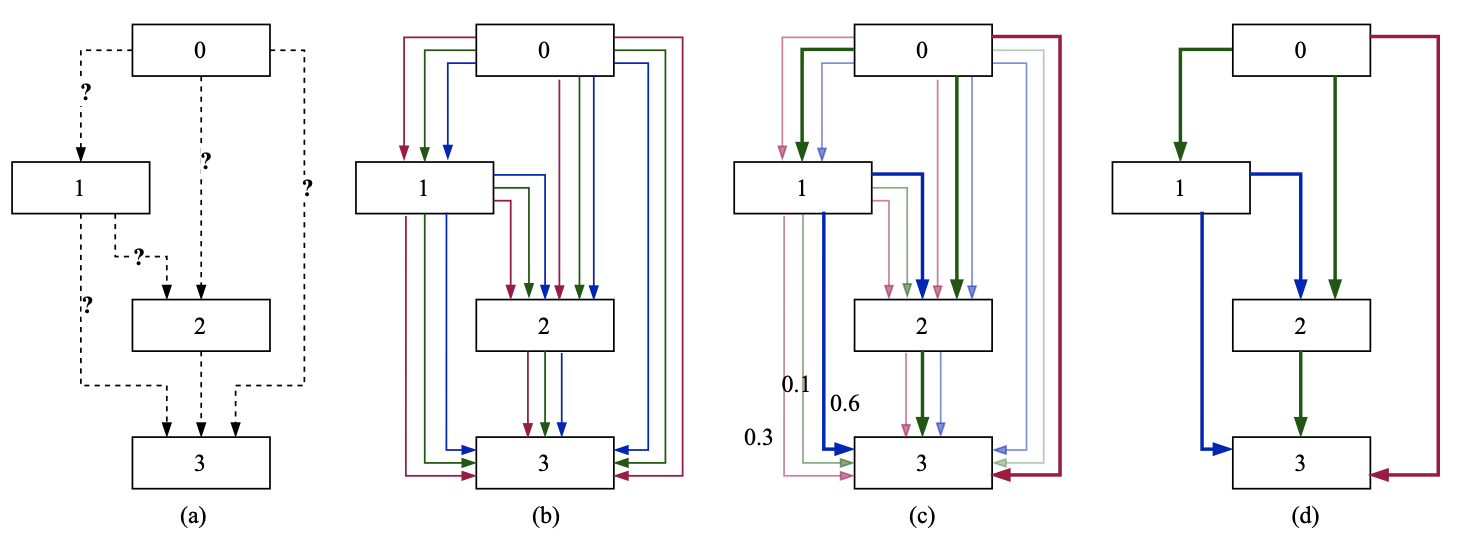
\includegraphics[width=1.0\linewidth]{gd-based-ao.png}
        \caption{Схема работы DARTS. Изначально операции на рёбрах неизвестны (a). До начала обучения операция на каждом ребре~--- это среднее из всех операций-кандидатов (b). Веса операций-кандидатов обновляются в процессе обучения (c). В финальной архитектуре используется операция с наибольшим весом (d).~\cite{bibl:sota}}
        \label{fig:sgd-based-ao}
    \end{figure}

    \emph{Оптимизация на основе суррогатной модели (Surrogate Model-based Optimization).}
    Идея подхода SMBO заключается в том, чтобы построить суррогатную модель, которая будет учитывать результаты оценки качества предыдущих архитектур и на основе их предсказывать наиболее многообещающую архитектуру.
    Таким образом, эти методы могут существенно сократить время поиска и повысить эффективность.
    В качестве суррогатной модели часто используются методы баесовской оптимизации, нейронные сети и ансамбли.

    \emph{Случайный поиск и перебор по сетке.}
    Исследования показывают, что случайный поиск является неплохим бейзлайном, который, при использовании некоторых оптимизационных трюков может быть почти настолько же эффективным, как методы на основе обучения с подкреплением и другие подходы.

    \emph{Гибридные методы.}
    Так как каждый из вышеперечисленных подходов имеет свои достоинства и недостатки, некоторые исследователи предложили комбинировать их.

    \textbf{Генерация модели: оптимизация гиперпараметров.}
    Большая часть подходов использует одинаковый набор гиперпараметров для всех полученных моделей.
    Это означает, что после того как лучшая архитектура будет найдена, необходимо вручную настроить её гиперпараметры.
    Чтобы автоматизировать этот процесс, было предложено использовать такие подходы, как случайный поиск и перебор по сетке, методы баесовской оптимизации, а также методы на основе градиентного спуска.

    \textbf{Оценка модели.}
    После того как очередная архитектура была получена, модель необходимо обучить и оценить её качество, что требует больших вычислительных затрат.
    Бало предложено несколько методов оптимизации этого этапа.

    \emph{Низкая точность (Low fidelity).}
    Наиболее простым подходом является обучение модели лишь на части исходного датасета с уменьшенной размерностью (например, с меньшим разрешением в случае изображений).
    Также можно обучать упрощённую версию модели или использовать меньшее количество итераций обучения.

    \emph{Разделение весов (Weight sharing).}
    Использование одних и тех же весов для нескольких архитектур позволяет значительно ускорить процесс оценки модели.

    \emph{Суррогатные методы (Surrogate).}
    Использование суррогатной модели позволяет ускорить обучение и оценку полученных архитектур.

    \emph{Преждевременная остановка (Early stopping).}
    Изначально преждевременная остановка обучения использовалась в классическом МО для предотвращения переобучения; однако некоторые исследования показали, что её можно использовать для ускорения этапа оценки полученной архитектуры, заканчивая обучение модели, если для неё была предсказана недостаточная точность.

    \textbf{Открытые проблемы и дальнейшие направления для исследований.}
    На данный момент у методов NAS есть ряд нерешённых проблем.
    Например, все описанные выше подходы используют созданные людьми операции в качестве базовых, что вносить некоторую предвзятость в получаемую архитектуру.
    Авторы статьи \cite{bibl:az} предложили использовать в качестве базовых операций простые математические преобразования.
    Их подход способен генерировать сложные архитектуры с нуля.
    
    Ещё одной задачей является применение AutoML в большем числе сфер.
    Сейчас исследования в основном сконцентрированы на задаче классификации изображений и лишь некоторые исследования пытаются применить данный подход к другим задачам. 

    Получаемые архитектуры зачастую сложно интерпретируемы и не обоснованы математически.
    Улучшение интерпретируемости AutoML является ещё одним направлением для исследований.

    Также большой проблемой является воспроизводимость результатов. 
    Было предложено несколько датасетов для сравнения различных методов друг с другом (NAS-Bench-101, NAS-Bench-201, NAS-Bench-NLP), однако здесь всё ещё есть пространство для дальнейших исследований.

    Недостатком многих методов является низкая производительность.
    Кроме того, большинство из них требуют для обучения хорошо подготовленные размеченные данные без шумов.

    Многие исследования рассматривали поиск архитектуры и оптимизацию гиперпараметров как отдельные задачи, однако они пересекаются по используемым методам, поэтому их можно осуществлять одновременно.

    Главная цель AutoML~--- полностью автономный процесс разработки модели~--- всё ещё не достигнута, хотя такие инструменты, как TPOT, Auto-WEAK, Auto-Sklearn, Auto-Keras и NNI, позволяют автоматизировать некоторые его части.

    На данный момент большинство исследований концентрировались на решении конкретной задачи.
    Ещё одним направлением для исследований является разработка таких систем, которые могли бы легко дообучаться на новых данных, не забывая при этом старые знания.

\subsection{The evolved transformer}
    В данной статье авторы предлагают применить эволюционный поиск алгоритмов к задачам, связанным с обработкой языка.
    Чтобы ускорить вычисления был предложен новый метод последовательных динамических препятствий (Progressive Dynamic Hurdles).
    В итоге была получена новая архитектура <<развитый трансформер>> (evolved transformer), которая превосходит трансформеры, созданные людьми, в области перевода текста.

    \begin{figure}[t]
        \centering
        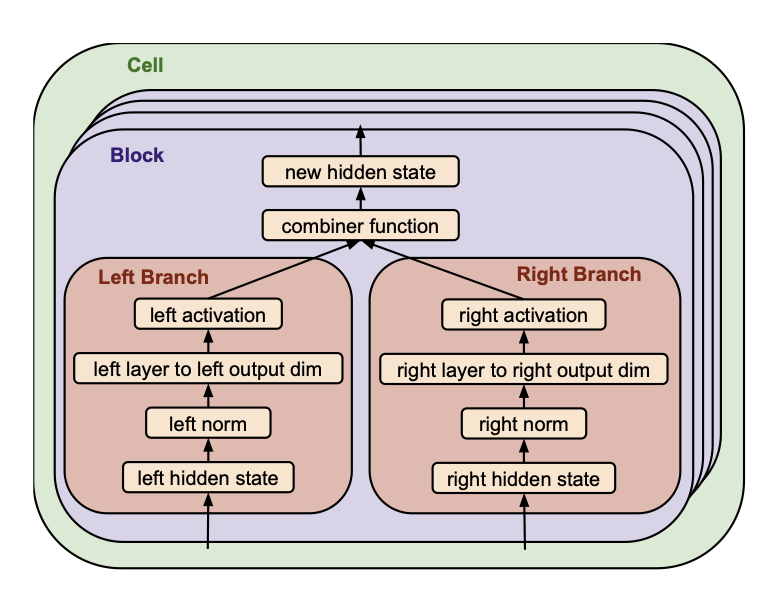
\includegraphics[width=0.5\linewidth]{evolved-transformer-search-space.png}
        \caption{Пространство поиска <<развитого трансформера>>.~\cite{bibl:evolved-transformer}.}
        \label{fig:et-search-space}
    \end{figure}


    Исследователи используют ячеистое пространство поиска.
    Архитектура представляется в виде нескольких ячеек, каждая из которых состоит из 6 (в случае энкодера) или 8 (в случае декодера) независимых блоков.
    Блок принимает на вход скрытые представления от предыдущих ячеек, обрабатывает их независимо, а затем комбинирует.
    Такое пространство поиска получается довольно большим, к тому же на обучение языковой модели требуется большое количество вычислительных ресурсов и времени.
    Чтобы решить эту проблему, исследователи предлагают две оптимизационные техники.
    Во-первых, в качестве начальной популяции используется уже зарекомендовавшая себя архитектура трансформера.

    Вторая техника была названа последовательными динамическими препятствиями (Progressive Dynamic Hurdles).
    Её суть заключается в том, что полное число шагов обучаются лишь наиболее успешные модели.
    Более конкретно, первые $m$ дочерние модели обучатся $s_0$ шагов, после чего вычисляется их средняя точность, которая объявляется препятствием $h_0$.
    Следующие $m$ моделей обучаются $s_0$ шагов, а затем ещё $s_1$ шагов, если их точность после оказалась больше $h_0$.
    Когда достаточное количество моделей обучилось на полном в течение $s_0 + s_1$ итераций, их средняя точность объявляется препятствием $h_1$, и так далее.

    В результате поиска была найдена архитектура развитого трансформера, которая превосходит своего предшественника в задачах машинного перевода текста.
    Сравнения производились на бенчмарках WMT 2014 English-German, WMT 2014 English-French (En-Fr), WMT 2014 English-Czech (En-Cs) и the 1 Billion Word Language Model Benchmark (LM1B).

\subsection{AutoML-Zero: Evolving Machine Learning Algorithms From Scratch}
    
    В данной статье авторы предлагают новый подход к генерации алгоритмов машинного обучения.
    До этого исследователи концентрировались на отдельных фрагментах алгоритма, таких как архитектура сети или используемые аугментации, сильно сужая пространство поиска или искажая результаты в пользу алгоритмов, схожих с теми, что создаются людьми (human bias).
    В новом исследовании авторы предлагают генерировать алгоритм целиком, включая предварительную инициализацию, способ обучения и формирования предсказания. На примере нескольких задач было показано, что генетические алгоритмы способны решать задачу поиска оптимального алгоритма в большом пространстве поиска, не только переизобретая известные алгоритмы, но и улучшая их.

    Алгоритмы представляются в виде программ, состоящих из трёх базовых функций: \texttt{Setup}, \texttt{Predict} и \texttt{Learn} (см. \figurename \ref{fig:az-code-exmpl}).
    Внутри каждой функции разрешено использование только базовых математических операций над скалярами, векторами и матрицами.
    Чтобы исключить генерацию схожих алгоритмов, ускорив тем самым поиск лучшего из них, был разработан способ сравнения таких программ, не учитывающий конкретную реализацию алгоритма (function equivalence checking, FEC).

    \begin{figure}[t]
        \centering
        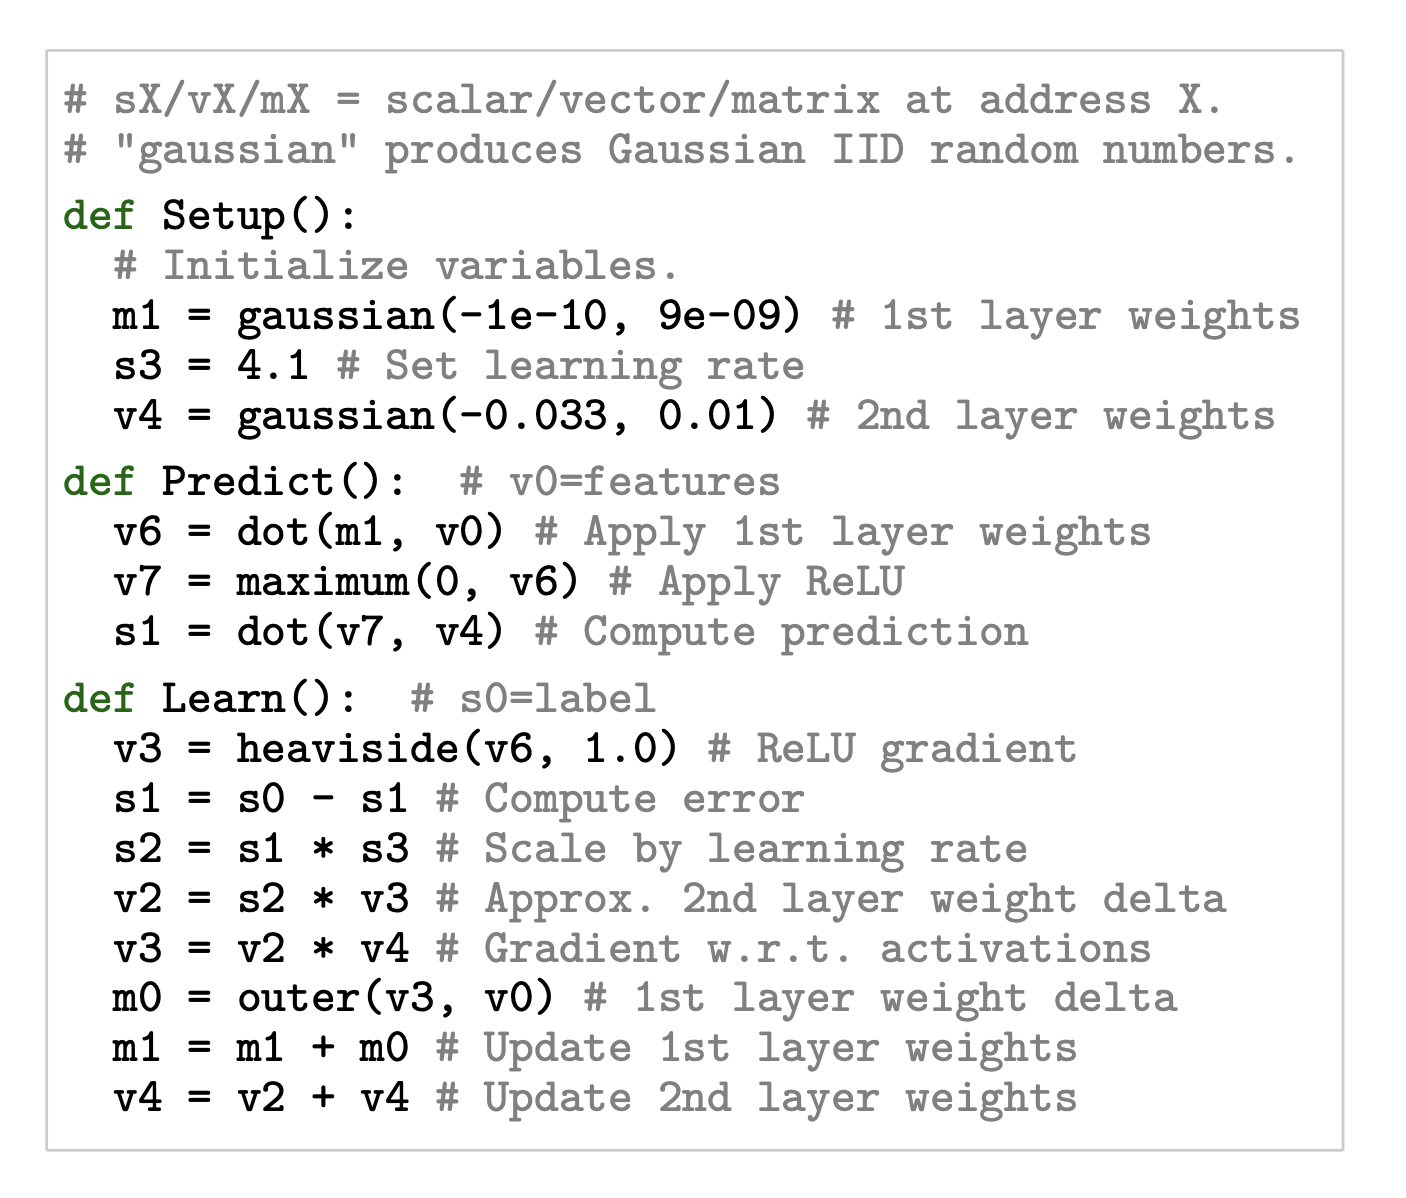
\includegraphics[width=0.7\linewidth]{auto_ml_zero_algoritm_example.png}
        \caption{Пример кода, полученного алгоритмом AutoML-Zero.~\cite{bibl:az}}
        \label{fig:az-code-exmpl}
    \end{figure}
    
    Поиск подходящего алгоритма производился с помощью генетического алгоритма.
    Для ускорения поиска были использованы два улучшения: вышеупомянутый FEC и метод последовательных препятствий~\cite{bibl:evolved-transformer}.
    Также использовался параллельный отбор нескольких популяций со случайной миграцией между ними.
    
    В ходе проведения нескольких экспериментов на задачах, таких как классификация изображений датасета CIFAR-10, выяснилось, что данный генетический алгоритм значительно лучше случайного поиска и способен создавать алгоритмы, превосходящие базовые решения, такие как линейная регрессия или полносвязные нейронные сети.
    Также в ходе эволюции удалось автоматически получить такие техники, как градиентный спуск и метод обратного распространения ошибки.
    Было показано, что при добавлении некоторых ограничений (малый объём данных или малое количество итераций обучения) генерируемые алгоритмы способны создавать адаптации к этим ограничениям.

    Таким образом, авторы предложили новый подход к Auto ML и способ его реализации.
    В качестве дальнейшего направления исследования авторы предлагают улучшение алгоритма поиска алгоритмов.
    Также авторы отмечают, что в их подходе имеются значительные недостатки: в текущей реализации появление таких алгоритмов, как свёрточные нейронные сети или batch normalisation, невозможно ввиду архитектурных ограничений.
    Исправление этих недостатков также оставляется для будущих исследований.

\subsection{MOAZ: A Multi-Objective AutoML-Zero Framework}
     
    Авторы данной статьи предлагают улучшение идеи, предложенной в статье AutoML-Zero (AZ).
    В отличие от своего предшественника, MOAZ старается оптимизировать не только точность получаемых алгоритмов, но и их эффективность, что важно для  большинства реальных применений.
    Использование двух целей также позволяет улучшить точность получаемых алгоритмов и упростить их, что значительно облегчает интерпретацию результата.

    Для реализации концепции многоцелевой оптимизации авторы статьи предложили следующие изменения.
    Например, была изменена оптимизируемая формула: берётся минимум из сложности алгоритма и ошибки с условием, что оба показателя не превышают максимально допустимые значения (сложность алгоритма определяется как суммарное число FLOPs в функциях \texttt{Setup}, \texttt{Learn} и \texttt{Predict}).
    Для оптимизации такой функции используется модификация алгоритма NSGA-II c изменёнными функциями выбора доминирующего кандидата и кроссинговера.

    \begin{figure}[t]
        \centering
        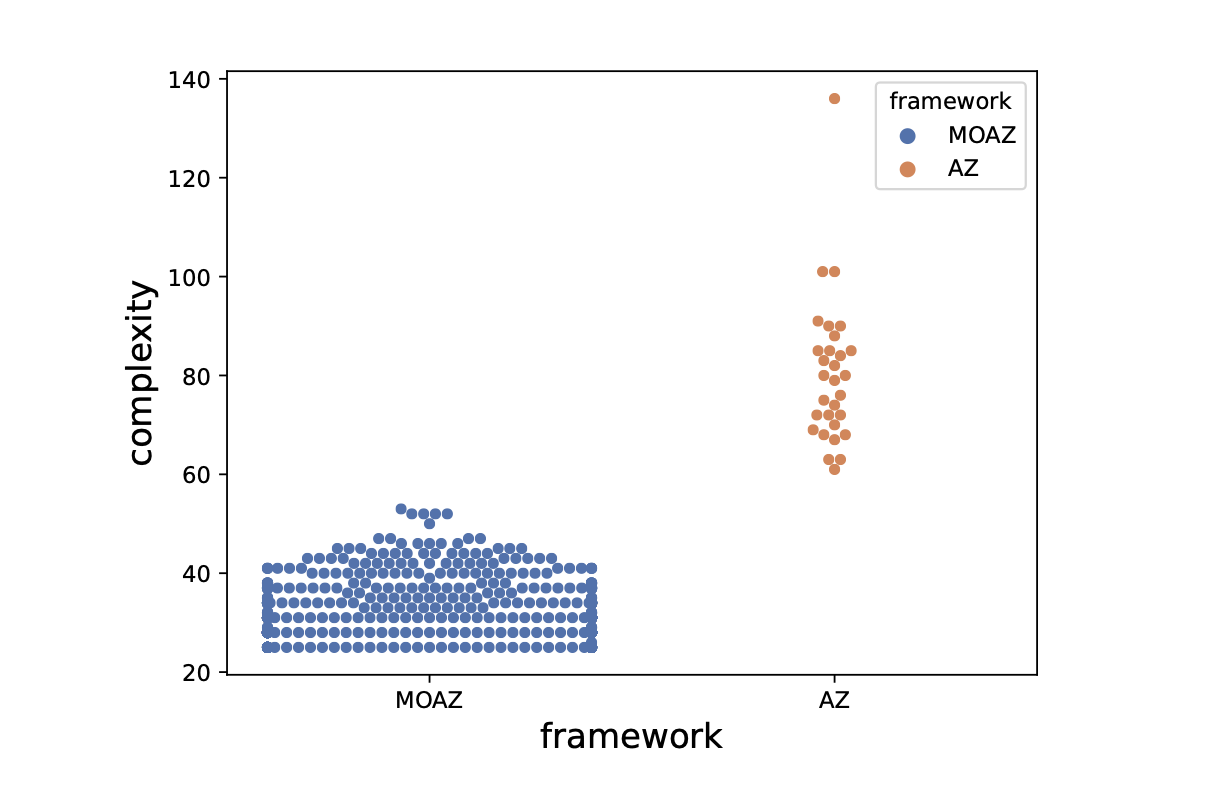
\includegraphics[scale=0.4]{moaz_and_az_complexity_comparizon.png}
        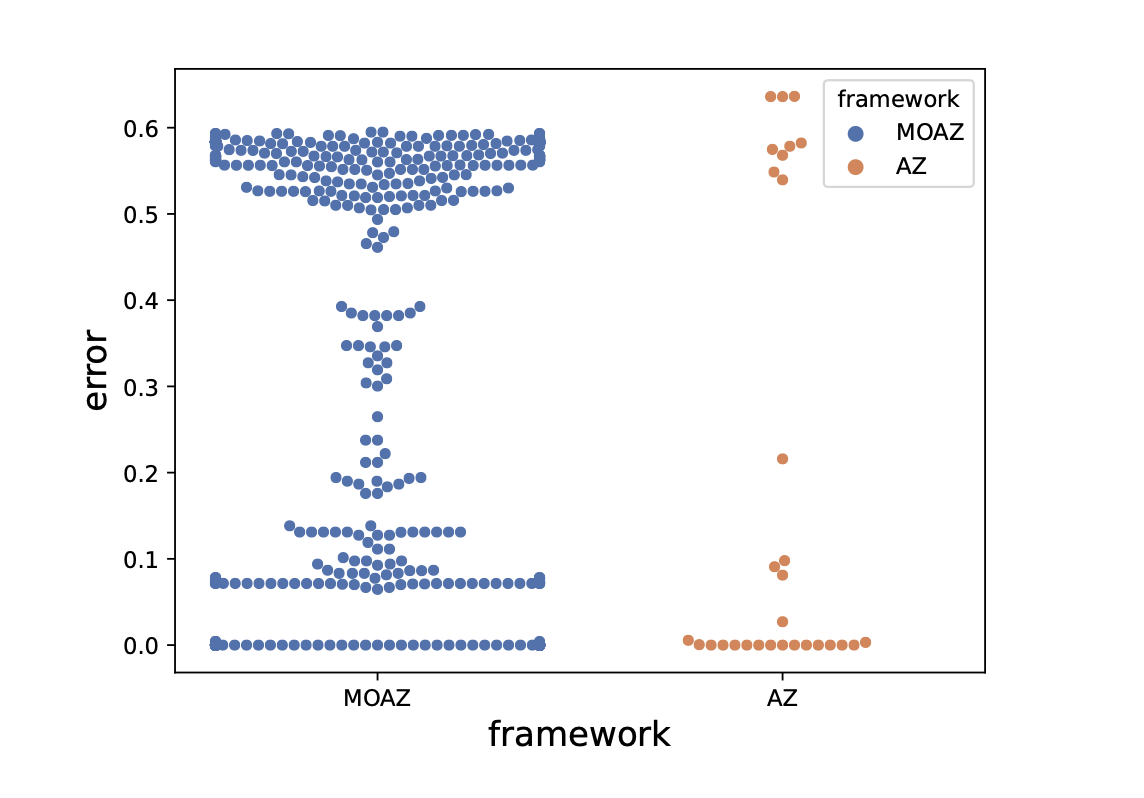
\includegraphics[scale=0.4]{moaz_and_az_error_comparizon.png}
        \caption{Сравнение сложности и ошибки алгоритмов, получаемых методами AZ и MOAZ.~\cite{bibl:moaz}}
        \label{fig:moaz_az_comp}
    \end{figure}

    В ходе запусков экспериментов было показано, что предложенный подход превосходит AZ не только в терминах сложности получаемых алгоритмов, но и по скорости и стабильности поиска достаточно хорошего решения (определяемого как решение с ошибкой меньше $10^{-1}$). 
    После тестирования на нескольких наборах искусственных задач было показано, что MOAZ находит достаточно хорошее решение для большего процента задач, причём количество  запусков до первого удачного решение сильно меньше, чем у AZ.

    Таким образом, предложенный в данной статье подход позволил получать алгоритмы сопоставимого качества (см.~\figurename~\ref{fig:moaz_az_comp}) быстрее и стабильнее, чем подход AZ.
    Полученные алгоритмы также эффективнее и легче поддаются интерпретации, что уменьшает нагрузку на человека на этапе постобработки полученного решения.
    Авторы статьи предлагают пути дальнейшего улучшения предложенного подхода путём добавления новых целей.

% \section{ZeroML: A Next Generation AutoML Language}
    

%     В данной статье авторы исследуют доступные библиотеки для реализации AutoML и при ходят к выводу, что все они имеют существенные недостатки.
%     Например, большинство из них используют низкопроизводительные языки высокого уровня, такие как Python или R.
%     К тому же для обучения моделей используются сторонние библиотеки, установка которых может быть затруднена из-за зависимостей или вообще недоступна для некоторых платформ.
%     Ещё одним недостатком является сложный ручной процесс запуска модели в продакшн.
%     Чтобы исправить эти и некоторые другие недостатки было предложено создать новый язык программирования, который имел бы встроенные механизмы для обучения моделей, был бы достаточно производительным и облегчал бы процесс выпуска модели.
    
%     Созданный язык программирования был назван ZeroML.
%     Его основные характеристики:
%     \begin{itemize}
%         \item \textbf{компилируемость}. Позволяет эффективно управлять ресурсами и устраняет многие недостатки интерепретируемых языков.
%         \item \textbf{мультипарадигмальность}. Сочетание процедурного и объектно-ориентированного программирования облегчает использование языка для людей с разным опытом программирования. 
%     \end{itemize}

    
%     \emph{P.S. В интернете нет информации про этот ЯП, все ссылки ведут либо на эту статью, либо на что-то явно другое. Также смущает отсутствие ссылок на какие-либо репозитории и несовпадение описания синтаксиса в разделе 7 с тем, что предоставлено в рис. 4. Возможно, придётся исключить.}

\newpage
\subsection{Alphaevolve: A coding agent for scientific and algorithmic discovery}

    В данной статье авторы предлагают агента для написания программ на основе LLM и эволюционного поиска.
    AlphaEvolve способен решать широкий спектр научных и инженерных задач, где решение может быть запущено и оценено автоматически.

    Процесс поиска решения является эволюционным алгоритмом и состоит из последовательных запусков следующего цикла:
    \begin{enumerate}
        \item Родительские программы извлекаются из базы данных
        \item На основе предложенных ранее решений и общего контекста задачи генерируется запрос к LLM 
        \item LLM предлагает свои правки к существующему решению
        \item Полученные решения автоматически оцениваются
        \item Наиболее успешные кандидаты записываются обратно в базу данных
    \end{enumerate}

    \begin{figure}[t]
        \centering
        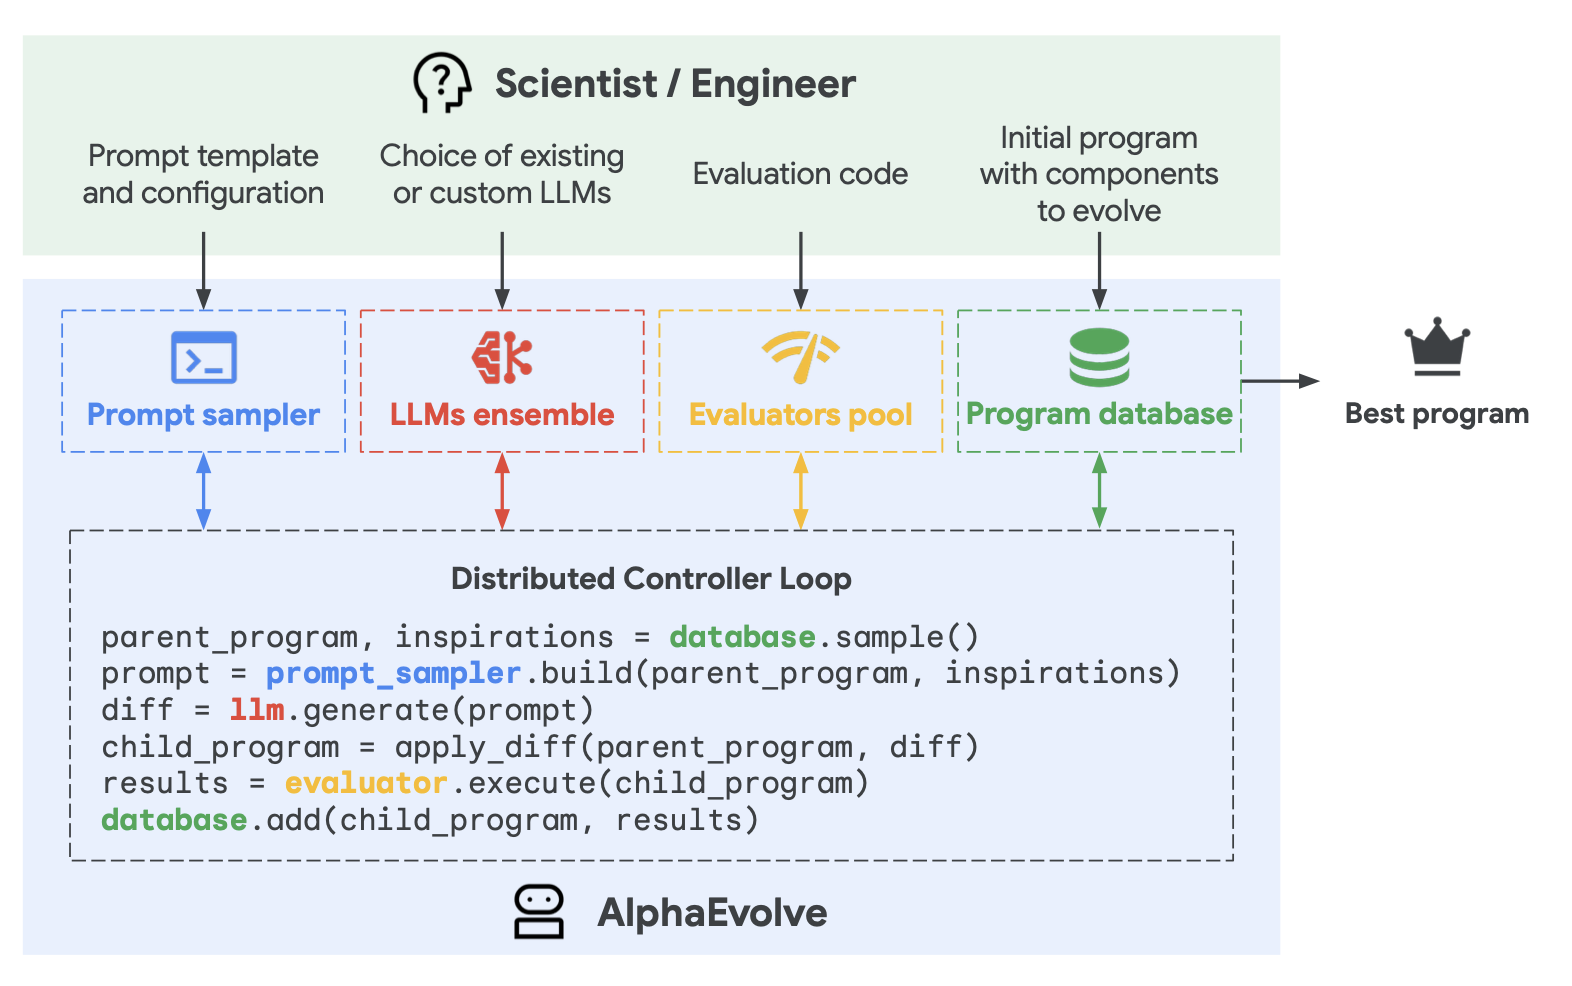
\includegraphics[width=\linewidth]{alphaevolve-discovery-process.png}
        \caption{Схема роботы AlphaEvolve.~\cite{bibl:alphaevolve}.}
        \label{fig:alphaevolve-discovery-process}
    \end{figure}

    AlphaEvolve может работать с целыми кодовыми базами.
    Конкретные участки, доступные для изменения, помечаются с помощью комментариев, что позволяет использовать агента, внося лишь незначительные правки в исходную кодовую базу.
    Также от пользователя требуется функция \texttt{evaluate()}, которая запускает решение и вычисляет значения метрик, которые необходимо оптимизировать.

    В ходе тестирования AlphaEvolve был запущен на множестве разнообразных задач: от открытых математических задач (быстрое перемножение матриц, проблема минимального перекрытия Эрдеша и т.п.) до практических задач по оптимизации вычислительной экосистемы компании Google (улучшенный алгоритм построения расписаний для дата-центров, оптимизация ядер нейросети Gemini и т. д.).
    Все эти задачи показали, что предложенный агент способен находить решения сложных задач и значительно улучшает возможности отдельных LLM.

\newpage
\subsection{ShinkaEvolve: Towards Open-Ended And Sample-Efficient Program Evolution}

    В данной статье предлагается новый подход к AutoML, основанный на применении LLM.
    Предложенный подход значительно эффективнее существовавших решений на базе LLM.
    Открытый исходный код открывает возможности для дальнейших экспериментов.

    ShinkaEvolve предлагает три основные архитектурные улучшения:
    \begin{enumerate}
        \item Смешанный выбор новых кандидатов (из родительской популяции и из архива лучших представителей данной популяции). Исследователи подчёркивают важность баланса между использованием уже зарекомендовавших себя подходов и поиском новых.
        \item Мутация кандидата осуществляется через предложение по улучшению от LLM. Недостаточно изменённые решения (используется сравнение эмбеддингов и оценка от LLM) отбраковываются.
        \item Изменённая процедура запуска и оценки качества нового решения
    \end{enumerate}
    
    Более подробно подход ShinkaEvolve заключается в следующем:
    
    \textbf{Отбор кандидатов}
    
    В архиве хранится фиксированное число программ с их точностью работы и мета информацией.
    Во время мутации БЯМ доступна программа из родительской популяции, несколько лучших, а также несколько случайных программ из архива.
    Популяция делится на <<острова>>, эволюционирующие по отдельности.
    Между островами возможна миграция; однако, чтобы поддерживать уникальность каждого из них, лучшее решение в каждой из популяций исключается из процесса миграции. 
    Исследователи также подчёркивают важность баланса между использованием эффективных подходов и поиском новых.
    Вероятность выбора программы в качестве родительской зависит от её точности, а также от количества и медианной точности её потомков.

    \textbf{Мутация кандидатов и оценка новизны}
    
    Перед запуском процесса эволюции выбирается набор LLM, которые будут осуществлять мутации, а также их параметры (температура, ограничение на использование размышлений и т.п.). 
    Представлены три вида мутаций:
    \begin{enumerate}
        \item Изменение отдельного блока программы
        \item Переписать программу с нуля
        \item Скрещивание программы с дополнительной программой из архива
    \end{enumerate}

    Оценка новизны производится следующим образом: сначала вычисляются эмбеддинги программ, которые затем сравниваются.
    Если похожесть двух программ превышает порог, то код отправляется LLM, которая оценивает, имеются ли существенные различия.

    \textbf{Запуск и оценка качества нового решения}
    
    После запуска каждого решения оно записывается в архив.
    К нему также добавляется информация о точности решения, а также набор заранее выбранных метрик вместе с текстовым отзывом о решении.
    Так как эффективность разных LLM может отличаться, для каждой LLM оценивается её вклад в улучшение качества решений (алгоритм UCB1); вероятность выбрать каждую модель в качестве мутатора зависит от этих параметров.
    ShinkaEvolve использует <<блокнот>> куда записываются описания всех решений, а также общие стратегии их оптимизации.
    Этого блокнот добавляется к каждому запросу на изменение программы.

    \begin{figure}[t]
        \centering
        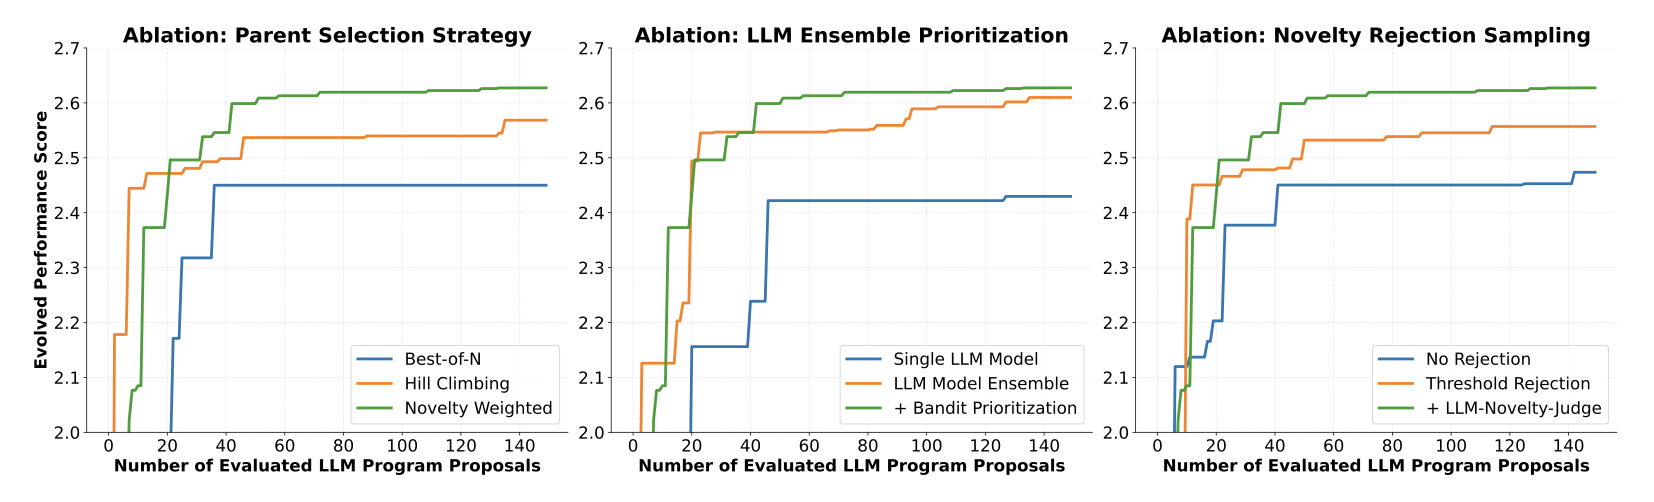
\includegraphics[width=1.0\linewidth]{shinkaevolve_analysis.png}
        \caption{Сравнение эффективности ShinkaEvolve без предложенных улучшений и с ними.~\cite{bibl:shinkaevolve}}
        \label{fig:shinkaevolve-ablation}
    \end{figure}

    Алгоритм ShinkaEvolve был протестирован на 4 задачах: упаковка кругов, AIME, ALE-Bench, задача обучения балансировщика для архитектуры MoE.
    На всех задачах алгоритм смог улучшить базовые решения.
    В одной из задач бенчмарка ALE-Bench ShinkaEvolve смог найти решение, занявшее второе место в рейтинге, а в последней задаче ShinkaEvolve предложил улучшение к популярной архитектуре балансировщика.
    Запуск на этих задачах показал, что почти все предложенные улучшения к алгоритму поиска решений дают значительное увеличение эффективности поиска.
    Исключение составляет только использование LLM для оценки новизны программ.
    Эксперименты показывают, что он даёт лишь незначительное улучшение по сравнению с эмбеддингами, что говорит о том, что одних только их уже достаточно для отсеивания слишком похожих кандидатов.

    Таким образом, авторы данной статьи предлагают новый подход, который оптимизирует использование LLM, позволяя значительно улучшить поиск решения.
    Авторы отмечают, что недостатками их подхода являются отсутствие возможности автоматической настройки баланса между использованием эффективных и поиском новых решений, а также ограниченный круг применимости из-за того, что подход заточен на цели в виде хорошо определённых числовых показателей.
    В качестве дальнейшего направления для исследований авторы видят устранение этих недостатков.
    
% \section{NGSA-II}
%     TODO
%     \emph{see: Kalyanmoy Deb, Amrit Pratap, Sameer Agarwal, and TAMT Meyarivan. A fast and elitist multiobjective genetic algorithm: Nsga-ii. IEEE Transactions on Evolutionary Computation, 6(2):182–197, 2002.}
    

% \section{Finite-time analysis of the multiarmed bandit problem}
%     TODO
%     \emph{See: Peter Auer, Nicolo Cesa-Bianchi, and Paul Fischer. Finite-time analysis of the multiarmed bandit problem. Machine learning, 47(2):235–256, 2002.}


\subsection{Automated design of agentic systems}

    Большие языковые модели часто используются в качестве агентов общего назначения.
    Несмотря на все успехи таких агентов, для многих задач требуется сложная система, имеющая доступ к внешним инструментам, таким как запуск кода или поисковая система.
    В результате было предложено много эффективных модулей для таких систем.
    Основываясь на опыте других областей машинного обучения, авторы данной статьи предлагают заменить ручную разработку отдельных модулей или даже агентов целиком их автоматической генерацией.
    Новая парадигма называется автоматическая разработка агентных систем (Automated Design of Agentic Systems, ADAS).
    Для решения данной задачи был предложен алгоритм мета-агентного поиска (Meta Agent Search), который в ходе экспериментов смог сгенерировать агента, превосходящего созданные вручную аналоги в задачах понимания текста и решения математических задач.

    Сначала авторы статьи определяют автоматическую разработку агентных систем как использование алгоритма поиска для нахождения агентных систем в пространстве поиска, которые оптимизируют целевую функцию.
    В данной работе в качестве пространства поиска используется пространство всех программ на некотором языке программирования.
    Такое пространство поиска позволяет найти любую возможную архитектуру агентной системы, а также предоставляет большую интерпретируемость по сравнению с другими пространствами.

    Чтобы найти новые успешные архитектуры в таком большом пространстве поиска был предложен алгоритм мета-агентного поиска.
    Он состоит из следующих шагов:
    \begin{enumerate}
        \item Архив инициализируется базовыми решениями (опционально)
        \item На основе архива генерируется новый агент: сначала высокоуровневое описание, а затем реализация в коде, после чего он проверяется на новизну
        \item Далее агент оценивается на валидационной выборке, проходя несколько итераций улучшения при необходимости
        \item Агент и информация о его работе на валидационной выборке добавляются в архив; процесс продолжается с обновлённым архивом, пока не будет достигнуто максимальное количество итераций
    \end{enumerate}

    \begin{figure}[t]
        \centering
        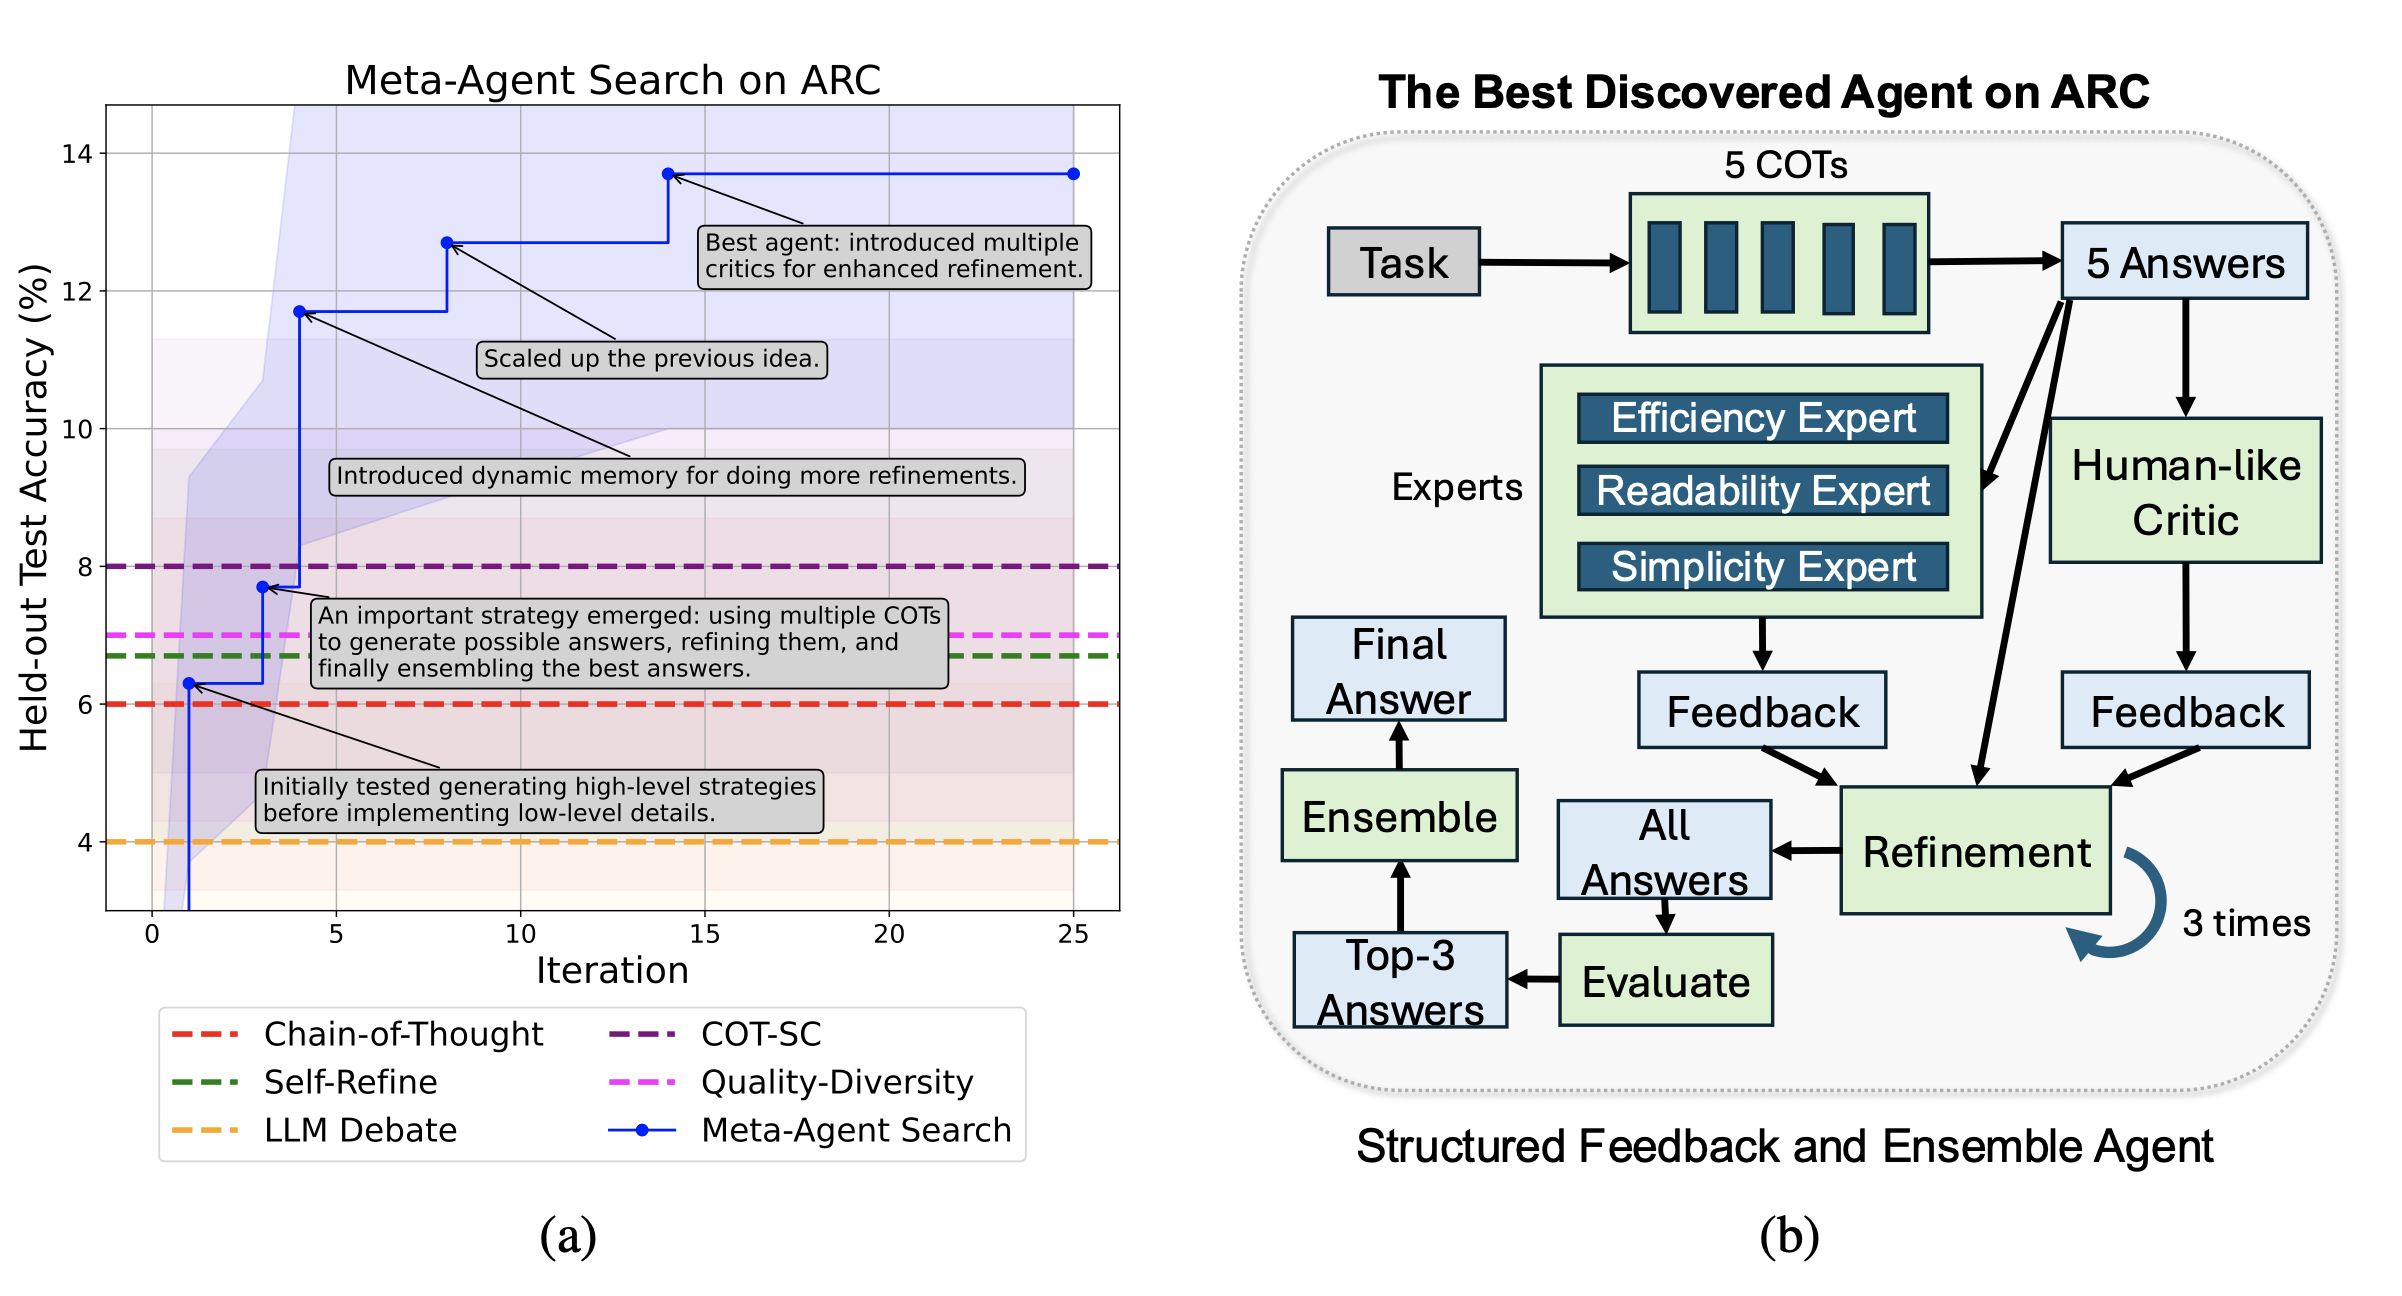
\includegraphics[width=\linewidth]{adas-arc-challenge-results.png}
        \centering
        \caption{Результат мета-агентного поиска для бенчмарка ARC: (a) мета-агентный поиск последовательно улучшает точность агента, (b) архитектура найденного агента.~\cite{bibl:adas}}
        \label{fig:adas-results}
    \end{figure}

    Исследователи провели эксперименты на бенчмарке Abstraction and Reasoning Corpus, четырёх бенчмарках для проверки способностей агентов в разных областях.
    Также была проверена возможность использовать агентов, созданных под математические задачи, для решения задач другого рода.
    Во всех экспериментах было обнаружено, что полученные агенты значительно превосходят аналоги созданные людьми, и сохраняют преимущество даже при использовании для других задач или с другой базовой моделью.

    Таким образом, в данной статье предлагается новое направление для исследований, а именно автоматическая разработка агентных систем.
    Было предложено пространство поиска в виде пространства программ на выбранном языке программирования, а в качестве метода поиска~--- мета-агентный поиск.
    Авторы обозначают множество направлений для дальнейших исследований: от предложений по улучшению алгоритма поиска до идей по практическому применению, например, дообучение агентов на новых данных, собранных после их запуска (Online Continual Learning).

\subsection{Ale-bench: A benchmark for long-horizon objective-driven algorithm engineering}
    Авторы данной статьи предлагают новый бенчмарк для оценки способности LLM генерировать решения алгоритмических задач.
    В отличие от предыдущих бенчмарков, использовавших задачи с заранее известным ответом, здесь используются более сложные задачи, а именно задачи на оптимизацию, точный оптимум которых недостижим.
    Это позволяет адекватно оценивать ИИ-системы, для которых задачи первого типа становятся слишком простыми.

    Бенчмарк представляет из себя датасет из 10 задач в облегчённой или 40 задач в полной версии, взятых с туров AtCoder Heuristic Contest.
    К каждой задаче прилагается условие, программа-оценщик, визуализатор поведения отправленного решения и лидерборда.
    Так как бенчмарк создавался в партнёрстве с AtCoder, все данные предоставлены официально, что гарантирует безопасное использование бенчмарка. 

    Бенчмарк реализован в качестве библиотеки на ЯП Python, цель которой состоит в том, чтобы позволить ИИ-системам решать задачи в формате, максимально приближенном к реальным AHC.
    Ключевую роль здесь играет объект \texttt{Session}, который запускает таймер контеста и предоставляет ИИ-системе протокол взаимодействия с тестирующей системой.
    ИИ может выполнять любое из 4 действий:
    \begin{enumerate}
        \item Просматривать условие задачи
        \item Запустить решение на открытых тестах, чтобы проверить решение
        \item Визуализировать работу решения
        \item Отправить финальный вариант решения
    \end{enumerate}
    После выполнения действия 4 или окончания времени сессия завершается, и объект \texttt{Session} выдаёт оценку решения на закрытых тестах.

    По результатам запусков ИИ-системы формируется несколько метрик.
    Первая группа вычисляется для каждой задачи отдельно:
    \begin{enumerate}
        \item Счёт в конкретной задаче 
        \item Ранг (rank)~--- место в рейтинге
        \item Результативность (performance)~--- метрика, вычисляемая через счёт и ранг по алгоритму Elo-rating.
    \end{enumerate}
    Вторая группа считается по всем задачам:
    \begin{enumerate}
        \item Средняя результативность по всем задачам 
        \item Рейтинг по системе, которая используется на настоящих AHC
    \end{enumerate}
    Авторы отмечают, что рейтинг может необъективно оценивать модель, так как одно крайне успешное участие может завысить общий рейтинг ИИ-системы.
    К тому же использование средней результативности вместе с её распределением по задачам позволяет выявить, насколько широк спектр задач, в которых ИИ показывает достойные результаты.

    Также в данной статье в качестве бэйзлайна была предложена система Ale-Agent.
    Ale-Agent использует две техники: запросы с общим знанием о задаче (в запросе к LLM сразу прилагаются стандартные идеи для решения задач такого типа) и ориентированный на разнообразие поиск решения.

    \begin{figure}[t]
        \centering
        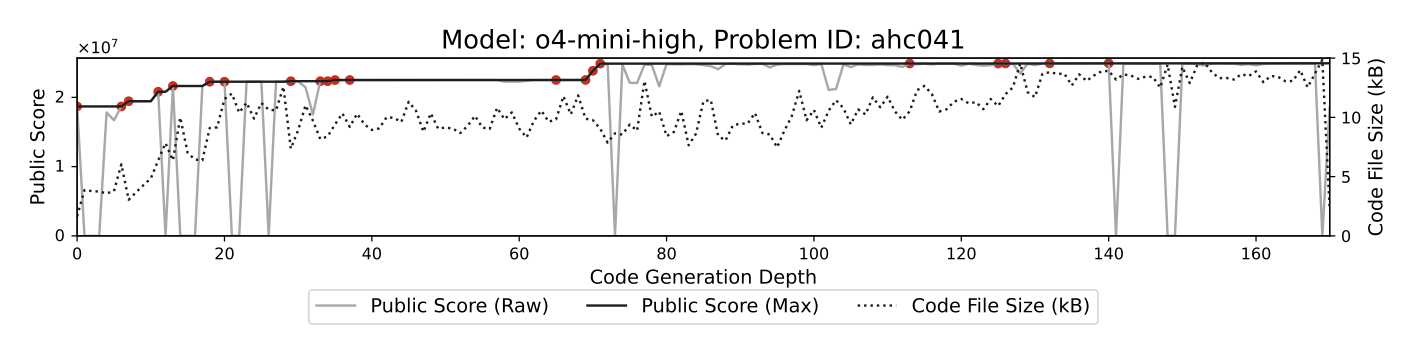
\includegraphics[width=1.0\linewidth]{ale-bench-o4-high-solving-progress.png}
        \caption{Прогресс модели 04-high в решении конкретной задачи. \cite{bibl:alebench}.}
        \label{fig:ale-bench-solving-progress}
    \end{figure}

    На данном бенчмарке было проведено множество экспериментов с разными моделями и стратегиями их использования.
    В первом эксперименте моделям давали всего одну попытку.
    Самой результативной оказалась модель 03-high, будучи единственной моделью со средней результативностью белее 1000.
    Ни одна из моделей не достигла результативности 2000 в какой-либо из задач, что подчёркивает сложность бенчмарка.

    Во втором эксперименте использовалась стратегия итеративного улучшения.
    Четыре модели (o4-mini-high, GPT-4.1 mini, DeepSeek-R1, Gemini 2.5 Pro) в течение 4 часов последовательно улучшали свои решения.
    В итоге самой результативной моделью оказалась o4-mini-high (средняя производительность 1520 и ). Модели o4-mini-high и GPT-4.1 mini были единственными, достигшими результативности хотя бы 400 на всех задачах, при этом последняя имеет меньший процент задач с результативностью хотя бы 2000 и меньшую среднюю результативность, чем DeepSeek-R1.

    По результатам экспериментов рейтинг модели o4-mini-high сопоставим с лучшими 11.8\% людей.
    Однако, если посмотреть на другие показатели, например, долю задач, где была достигнута результативность 1600 или 2400, то в среднем эти показатели значительно выше у людей.
    Это показывает, почему рейтинг не самый информативный показатель применительно к языковым моделям.

    Ещё один эксперимент сравнивал стратегию последовательного улучшения со стратегией <<параллельного поиска>> (многократный запуск бенчмарка с одной попыткой на задачу).
    В результате стратегия последовательного улучшения приводила к значительно большей результативности.
    Это говорит о том, что стратегия многих попыток не приводит к хорошим результатам на бенчмарке Ale-Bench.
    Чтобы достичь большой результативности, нужно последовательно улучшать решения, основываясь на предоставляемой обратной связи.

    По результатам экспериментов не было обнаружено связи между датой, где заканчивались знания модели, и её результативностью на задачах.
    Также в решениях моделей не было найдено признаков плагиата.

    Таким образом, в данной статье был предложен бенчмарк Ale-Bench, который проверяет способность ИИ-систем создавать и улучшать алгоритмы.
    Основным недостатком бенчмарка исследователи называют малое число задач.
    В качестве дальнейшего направления работы предлагается использование LLM для синтеза новых задач, что позволит уменьшить риск переобучения тестируемых ИИ-систем под конкретные типы и формулировки задач.
    
\newpage
\section{Доступные датасеты и бенчмарки}
    Так как целью AutoML было автоматизировать процесс разработки модели для решения конкретных задач, то для оценки используются датасети для этой задачи.
    Изначально автоматическое машинное обучение применялось преимущественно к задаче классификации изображений, поэтому для оценки использовались стандартные для области компьютерного зрения датасеты, такие как MNIST, CIFAR-10, ImageNet и т.п.
    Затем подходы AutoML начали применять и к другим областям.
    Для оценки решения в области обработки языка могут использоваться WMT 2014 English-German, WMT 2014 English-French, WMT 2014 English-Czech или the 1 Billion Word Language Model Benchmark, а например, агентов оценивают на бенчмарках Abstraction and Reasoning Corpus, DROP, MGSM, MMLU и GPQA.

    Однако использование таких датасетов создаёт трудности при сравнении двух систем, если для их оценки использовались разные датасеты.
    Также эксперименты могут различаться по используемым гиперпараметрам, вычислительным ресурсам и т.п.
    Чтобы исправить эту проблему были предложены специализированные датасеты, такие как NAS-Bench-101, NAS-Bench-201 для задачи классификации изображений и NAS-Bench-NLP для задач из области автоматической обработки языка.
    
    Ещё одна группа бенчмарков позволяет сравнивать способности языковых моделей генерировать решения алгоритмических задач.
    Среди них такие бенчмарки, как CodeContests, LiveCodeBench и Ale-Bench.
    Более подробное описание последнего было представлено ранее. 

\section{Постановка задачи и дальнейший план работы}
    % В рамках работы планируется создать агента для оптимизации целевой функции.
    % Агент будет использовать запросы к заранее выбранному множеству больших языковых моделей, чтобы строить оптимизатор как комбинацию известных алгоритмов и эвристик.

    % В качестве функций для оптимизации будут использоваться функции из бенчмарка COCO (подробное описание можно увидеть в статье~\cite{bibl:coco}).
    % Будут использоваться готовые реализации эвристик из библиотеки Opytimizer (описание представлено в статье \cite{bibl:opytimizer}).
    % Создавать оптимизатор планируется с помощью алгоритма, основанном на запросах к языковым моделям с исходным кодом или предоставляющим возможность обращаться к ним через API.
    % Полный список языковых моделей, которые будут использоваться для генерации оптимизаторов, будет составлен позднее.

    % Исходя из этого, план дальнейшей работы выглядит следующим образом:
    % \begin{enumerate}
    %     \item Подготовить список используемых LLM
    %     \item Составить алгоритм генерации оптимизатора целевой функции
    %     \item Реализовать агента для оптимизации целевой функции
    %     \item Оценить качество работы агента с помощью функций из бенчмарка COCO 
    % \end{enumerate}


    В рамках данной работы планируется создать агента для автоматической генерации оптимизатора заранее выбранной целевой функции.
    Основываясь на подходах, описанных в статьях \cite{bibl:alphaevolve} и \cite{bibl:shinkaevolve}, мы будем использовать генетический алгоритм с большими языковыми моделями в качестве источника мутаций, так как этот подход является одним из самых эффективных на данный момент.
    Чтобы сократить пространство поиска, мы будем использовать эвристики из библиотеки Opytimizer~\cite{bibl:opytimizer} в качестве элементов, из которых будет строиться оптимизатор.
    Будут использоваться целевые функции из бенчмарка COCO~\cite{bibl:coco}.


\subsection{Целевая функция. Бенчмарк COCO}
    \begin{figure}
        \centering
        \subfigure[]{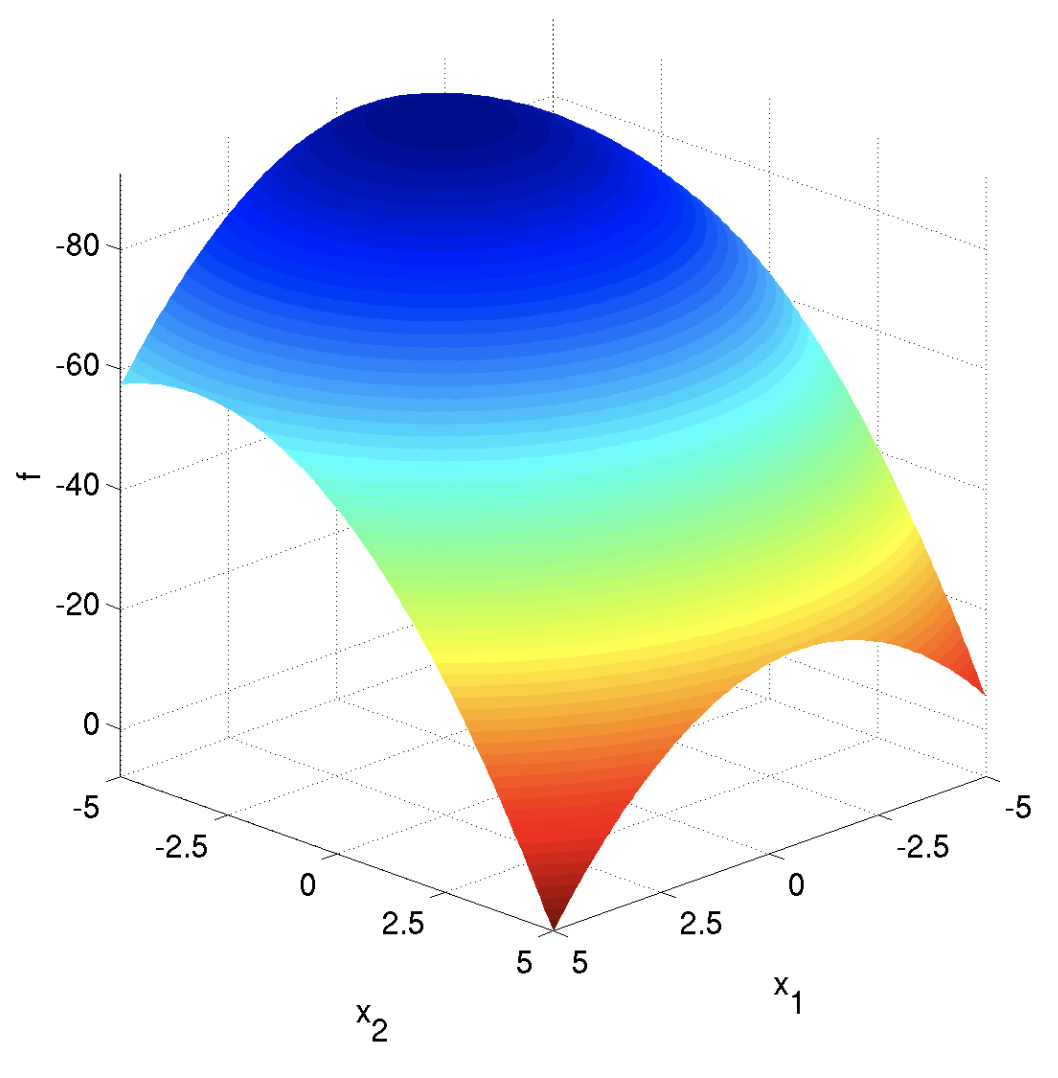
\includegraphics[width=0.3\textwidth]{spherical.png}}
        \subfigure[]{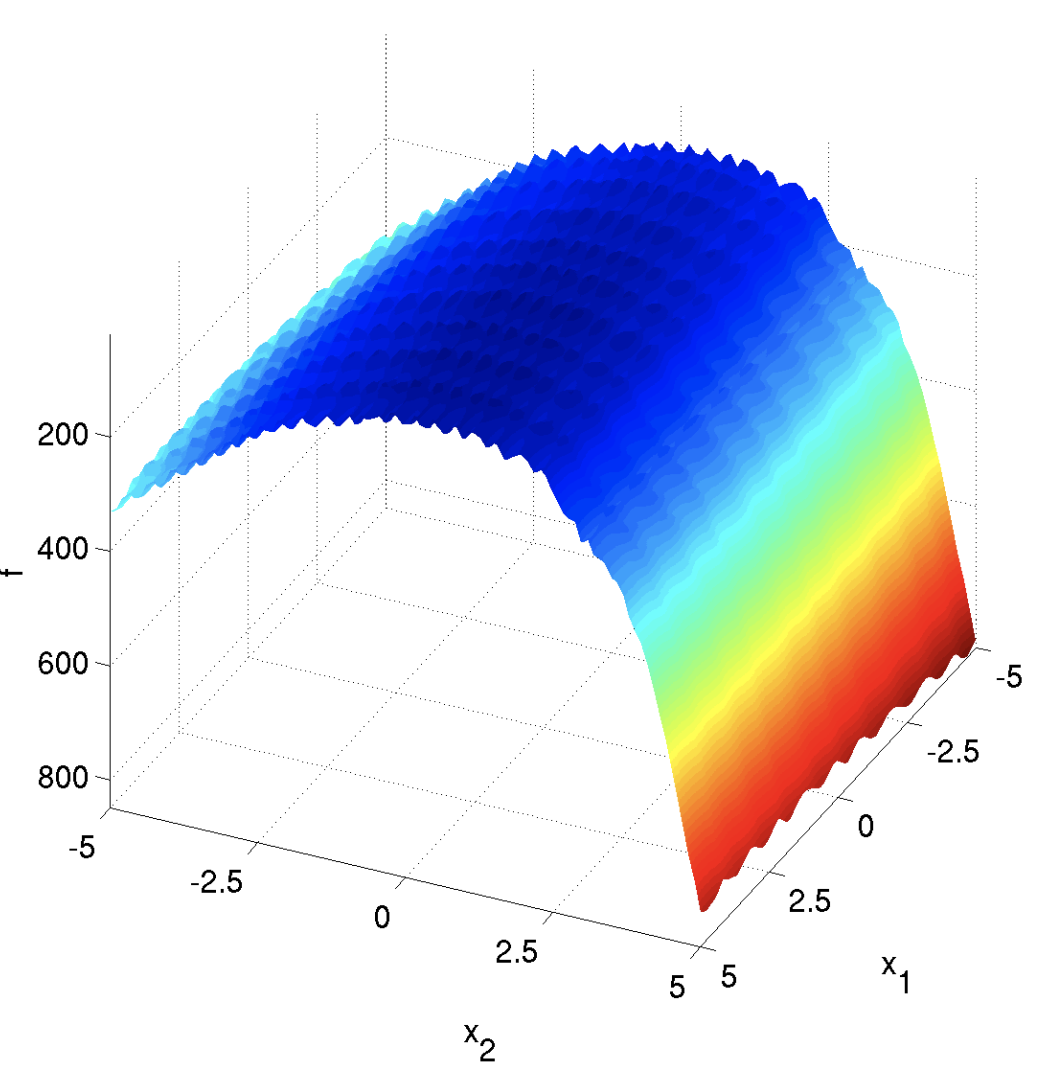
\includegraphics[width=0.3\textwidth]{rastrigin.png}}
        \subfigure[]{ 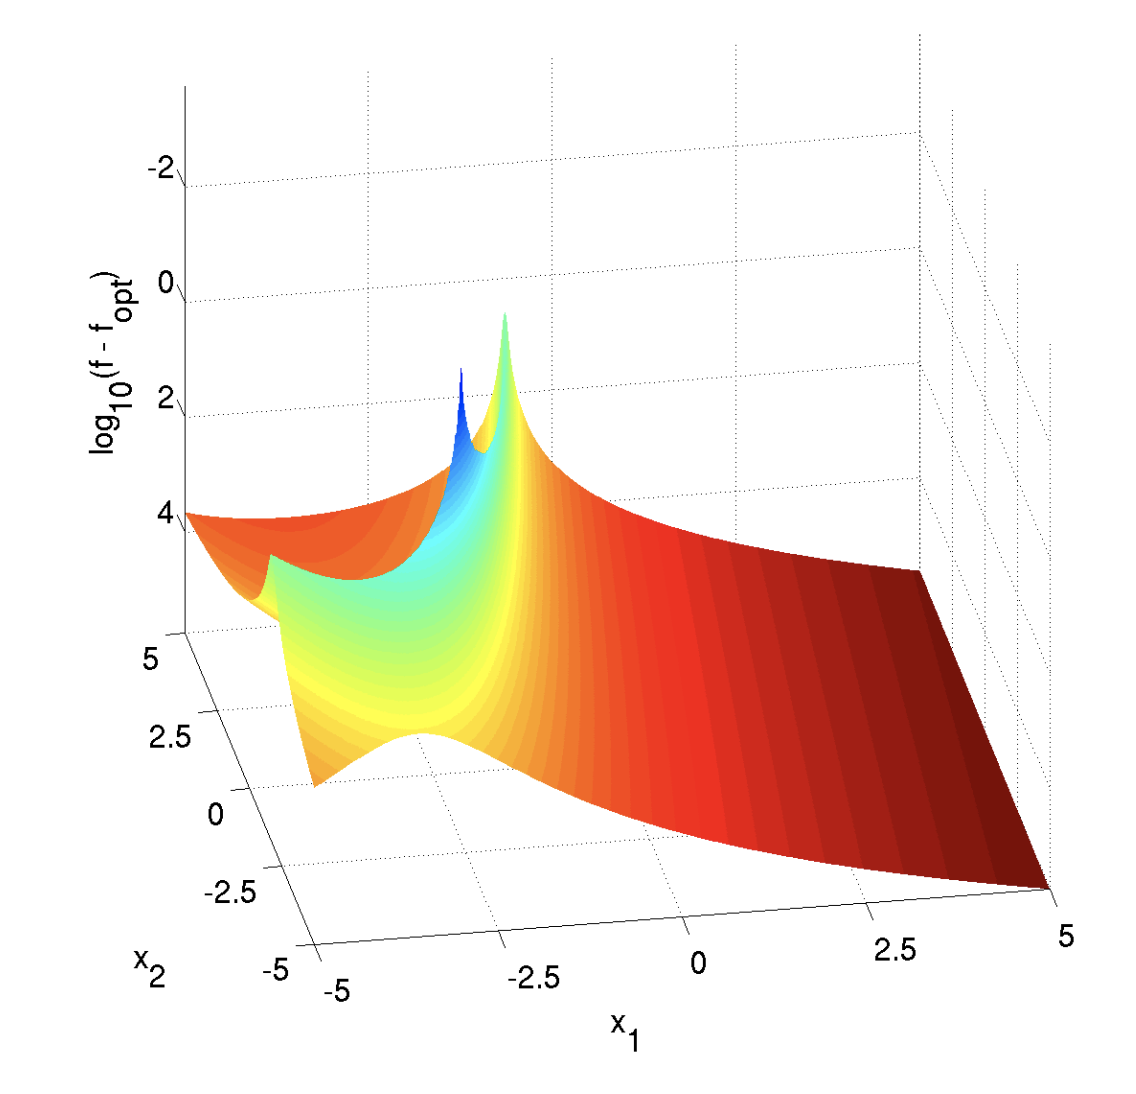
\includegraphics[width=0.3\textwidth]{rosenbrock.png}}
        \caption{Примеры функций для оптимизации из бенчмарка COCO: (a) сферическая функция, (b) функция Растригина, (c) функция Розенброка.~\cite{bibl:functions}}
        \label{fig:functions}
    \end{figure}
    Бенчмарк COCO был создан для автоматизации трудоёмкой и повторяющейся работы по оценке качества работы оптимизаторов.
    Основными понятиями COCO являются:
    \begin{itemize}
        \item Функция~--- класс отображений, устроенный схожим образом
        \item  Инстанс~--- конкретная реализация функции
        \item  Целевое значение~--- заранее оценённое как оптимальное значение индикатора качества
        \item Время работы~--- количество вызовов целевой функции перед достижением целевого значения
        \item Задача~--- совокупность конкретного инстанса, на котором запускается оптимизатор, и целевого значения
        \item Набор тестов~--- коллекция проблем
    \end{itemize}
    
    В рамках нашей работы целью будет \emph{разработать метод автоматического синтеза оптимизатора, имеющего минимально возможное среднее ожидаемое время работы на заданном наборе тестов}.

    COCO предоставляет несколько наборов тестов, отличающихся по размерности, количеству целей, зашумлённости и т.д.
    Мы будем использовать самый стандартный набор bbob, который содержит 24 незашумлённые функции.
    Функции разделены на 5 групп по сложности их оптимизации.
    Примеры функций из этого нобора представлены на \figurename~\ref{fig:functions}.
    
\subsection{Пространство поиска. Библиотека Opytimizer}
    Opytimizer~--- это библиотека с открытым кодом на Python для оптимизации целевых функций с помощью мета-эвристик.
    Opytimizer предоставляет почти 90 различных мета-эвристик 7 различных типов (эволюционные алгоритмы, алгоритмы на основе роевого интеллекта, на основе природных явлений и др.), предоставляющих единое API.
    Примеры алгоритмов из Opytimizer:
    \begin{itemize}
        \item Поиск гармонии (Harmony search)~--- эволюционный алгоритм, вдохновлённый процессом музыкальной импровизации.
        \item Алгоритм водного цикла (Water cycle algorithm)~--- алгоритм на основе имитации природных явлений, а именно  процесса формирования рек.
        \item Алгоритм летучих мышей (Bat algorithm)~--- алгоритм роевого интеллекта, вдохновлённый эхолокацией летучих мышей.
    \end{itemize}

    В рамках данной работы библиотека будет выступать в качестве источника примитивов~--- наборов готовых алгоритмов, которые агент сможет комбинировать.
    Хотя набор функций большой, он всё же конечен, что обуславливает необходимость их комбинации для достижения лучших результатов на конкретных задачах.
    Стандартизированный API позволяет автоматически валидировать сгенерированный код, а возможности для визуализации дают обратную связь о поведении синтезированного алгоритма.
    
\subsection{Общая схема работы агента}
    Основная задача агента~--- на основе описания целевой функции из бенчмарка COCO и доступного каталога алгоритмов библиотеки Opyrimizer, сгенерировать оптимизатор, который минимизирует ожидаемое время работы на заданном классе функций.
    %Примерный алгоритм работы представлен в алгоритме~\ref{alg:agent}.

    Для синтеза оптимизатора будут использоваться языковые модели, предоставляющие доступ по API, а также модели с открытым исходным кодом, которые можно развернуть локально.
    При выборе моделей будут учитываться такие показатели, как качество генерации кода (может оцениваться по бенчмаркам, например, HumanEval или MBPP), способность к исправлению ошибок, доступность (стоимость запроса для облачных моделей; наличие открытых весов, требования к видеокарте для локальных моделей).
    Конкретный список моделей будет сформирован позднее.
    
   % \input{codeps}

\newpage
\begin{thebibliography}{100}
    \bibitem{bibl:az} Esteban Real, Chen Liang, David So, and Quoc Le. AutoML-zero: Evolving machine learning algorithms from scratch. In Hal Daumé III and Aarti Singh, editors, Proceedings of the 37th International Conference on Machine Learning, volume 119 of Proceedings of Machine Learning Research, pages 8007–8019. PMLR, 13–18 Jul 2020.
    \bibitem{bibl:moaz} Guha, Ritam, et al. Moaz: A multi-objective automl-zero framework. Proceedings of the Genetic and Evolutionary Computation Conference. 2023.
    \bibitem{bibl:evolved-transformer} So, D. R., Liang, C., and Le, Q. V. The evolved transformer. In ICML, 2019.
    \bibitem{bibl:ngsa} Kalyanmoy Deb, Amrit Pratap, Sameer Agarwal, and TAMT Meyarivan. A fast and elitist multiobjective genetic algorithm: Nsga-ii. IEEE Transactions on Evolutionary Computation, 6(2):182–197, 2002.
    % \bibitem{bibl:zeroml} ZeroML. TODO: \emph{source}
    \bibitem{bibl:shinkaevolve} Lange, Robert Tjarko, Yuki Imajuku, and Edoardo Cetin. Shinkaevolve: Towards open-ended and sample-efficient program evolution. arXiv preprint arXiv:2509.19349 (2025).
    \bibitem{bibl:alphaevolve} AlexanderNovikov, NganVu, MarvinEisenberger, EmilienDupont, Po-SenHuang, AdamZsoltWagner, Sergey Shirobokov, Borislav Kozlovskii, Francisco JR Ruiz, Abbas Mehrabian, et al. Alphaevolve: A coding agent for scientific and algorithmic discovery. arXiv preprint arXiv:2506.13131, 2025.
    \bibitem{bibl:bandit} Peter Auer, Nicolo Cesa-Bianchi, and Paul Fischer. Finite-time analysis of the multiarmed bandit problem. Machine learning, 47(2):235–256, 2002.
    \bibitem{bibl:adas} Shengran Hu, Cong Lu, and Jeff Clune. Automated design of agentic systems. arXiv preprint arXiv:2408.08435, 2024.
    \bibitem{bibl:alebench} Yuki Imajuku, Kohki Horie, Yoichi Iwata, Kensho Aoki, Naohiro Takahashi, and Takuya Akiba. Ale-bench: A benchmark for long-horizon objective-driven algorithm engineering. arXiv preprint arXiv:2506.09050, 2025.
    \bibitem{bibl:sota} He, Xin, Kaiyong Zhao, and Xiaowen Chu. AutoML: A survey of the state-of-the-art. Knowledge-based systems 212 (2021): 106622.
    \bibitem{bibl:first-automl} B. Zoph, Q. V. Le, Neural architecture search with reinforcement learning, in: 5th International Conference on Learning Representations, ICLR 2017, Toulon, France, April 24-26, 2017, Conference Track Proceedings, OpenReview.net, 2017.
    \bibitem{bibl:clean1} I. F. Ilyas, Effective data cleaning with continuous evaluation., IEEE Data Eng. Bull. 39 (2) (2016) 38–46.
    \bibitem{bibl:clean2} M. Mahdavi, F. Neutatz, L. Visengeriyeva, Z. Abedjan, Towards automated data cleaning workflows, Machine Learning 15 (2019) 16.
    \bibitem{bibl:morphism} T. Wei, C. Wang, Y. Rui, C. W. Chen, Network morphism, in: M. Balcan, K. Q. Weinberger (Eds.), Proceedings of the 33nd International Conference on Machine Learning, ICML 2016, New York City, NY, USA, June 19-24, 2016, Vol. 48 of JMLR Workshop and Conference Proceedings, JMLR.org, 2016, pp. 564–572.
    \bibitem{bibl:rlautoml} B. Zoph, Q. V. Le, Neural architecture search with reinforcement learning, in: 5th International Conference on Learning Representations, ICLR 2017, Toulon, France, April 24-26, 2017, Conference Track Proceedings, OpenReview.net, 2017. URL https://openreview.net/forum?id=r1Ue8Hcxg
    \bibitem{bibl:coco} Nikolaus Hansen, Dimo Brockhoff, Olaf Mersmann, Tea Tusar, Dejan Tusar, Ouassim Ait ElHara, Phillipe R. Sampaio, Asma Atamna, Konstantinos Varelas, Umut Batu, Duc Manh Nguyen, Filip Matzner, Anne Auger. COmparing Continuous Optimizers: numbbo/COCO on Github. Zenodo, DOI:10.5281/zenodo.2594848, March 2019.
    \bibitem{bibl:opytimizer} de Rosa, Gustavo H., Douglas Rodrigues, and João P. Papa. "Opytimizer: A nature-inspired python optimizer." arXiv preprint arXiv:1912.13002 (2019).
    \bibitem{bibl:functions} Finck, Steffen, et al. Real-parameter black-box optimization benchmarking 2009: Presentation of the noiseless functions. Technical Report 2009/20, Research Center PPE, 2009. Updated February, 2010.
    
\end{thebibliography}

\end{document}
